\documentclass{beamer}
\usepackage[orientation=portrait,width=30in,height=40in,scale=1.35,debug]{beamerposter}
\mode<presentation>{\usetheme{ZH}}
\usepackage{chemformula}
\usepackage[utf8]{inputenc}
\usepackage[english]{babel} % required for rendering German special characters
\usepackage{hyperref} %enable hyperlink for urls
\usepackage{ragged2e}
\usepackage[font=small, justification=justified]{caption}
\usepackage{array,booktabs,tabularx}
\usepackage{bm}
\usepackage{natbib}
\bibliographystyle{abbrvnat}
\usepackage{subcaption}

\def\ci{\perp\!\!\!\!\!\perp}

\newcolumntype{Z}{>{\centering\arraybackslash}X} % centered tabularx columns
\title{\huge A Generalized Parameterization for \\ Mixed Data Linear Structural Equation Models}
\author{Ankur Ankan, Johannes Textor}
\institute[RU]{Institute for Computing and Information Sciences \\ Radboud University, Netherlands}
\date{\today}

% edit this depending on how tall your header is. We should make this scaling automatic :-/
\newlength{\columnheight}
\setlength{\columnheight}{106cm}

\begin{document}
\begin{frame}
\begin{columns}
	\begin{column}{.33\textwidth}
		\begin{beamercolorbox}[center]{postercolumn}
			\begin{minipage}{.98\textwidth}  % tweaks the width, makes a new \textwidth
				\parbox[t][\columnheight]{\textwidth}{ % must be some better way to set the the height, width and textwidth simultaneously
	\begin{myblock}{Introduction}
		\begin{figure}
			\includegraphics[page=1, scale=4]{figures.pdf}
			\caption{Example of an SEM. The variables $ \{ X_1, X_2, X_3, X_4 \} $ are continuous with path coefficients denoted by $ \beta_{ij} $.}
			\label{fig:example_sem}
		\end{figure}

		\vspace{1em}
		
		Continuous variable linear Structural Equation Models (SEMs)
		are parameterized using \textbf{path coefficients}, defined as
		the coefficients of a multiple regression model of each
		variable on its parents after scaling all variables to unit
		variance. Path coefficients are \textbf{interpretable}:
		\begin{itemize}
			\item One unit change in $ X_2 $ while keeping $ X_4 $ fixed implies $ \beta_{23} $ change in $ X_3 $. 
			\item Wright's path tracing rules \citep{Wright1934}
				can be applied. For example, the indirect
				effect of $ X_2 $ on $ X_3 $ is $ \beta_{24}
				\beta_{34} $, and the total effect of $ X_2 $ on
				$ X_3 $ is $ \beta_{24} \beta_{34} + \beta_{23}
				$.
		\end{itemize}

		\begin{figure}
			\includegraphics[page=4, scale=4]{figures.pdf}
			\caption{Example of a hypothesized mixed variable SEM
				based on the adult income dataset
				\citep{kohavi1996}. The variables Age and Hours
				Per Week are considered continuous, Education
				and Income are considered ordinal, and Sex and
				Occupation are considered categorical.}
			\label{fig:example_adult}
		\end{figure}

		\vspace{1em}

		However, such parameterization is \textbf{not available} for
		mixed data models (Fig.~\ref{fig:example_adult}). If regression
		based methods are used on mixed variables, we get a matrix of
		regression coefficients, which is not easily interpretable.

		\vspace{1em}

		\textbf{Research Question 1:} \textcolor{red}{Can we generalize path coefficients to mixed variable SEMs?}
	\end{myblock}\vfill
	\begin{myblock}{Path Coefficients and Effect Sizes}
		The parameter $ \beta_{23} $ in Fig.~\ref{fig:example_sem} can be estimated using the regression equation:
		
		\begin{equation*}
			X_3 \sim X_2 + X_4
		\end{equation*}
	
		The Frisch-Waugh-Lovell theorem \citep{Frisch1933} provides an alternative way to 
		estimate $ \beta_{23} $ in terms of the residuals of $ X_2 $ and $ X_3 $ while using the remaining covariates as the predictors.

		\begin{equation*}
			\begin{split}
				R_{X_2} &= X_2 - \mathbb{E}[X_2 | X_4] \\
				R_{X_3} &= X_3 - \mathbb{E}[X_3 | X_4] \\
				\hat{\beta}_{23} &: R_{X_3} \sim R_{X_2} \\
			\end{split}
		\end{equation*}

		This can be further reformulated in terms of the correlation coefficient, an effect size measure, between $ R_{X_2} $ and $ R_{X_3} $ as:

		\begin{equation*}
			\hat{\beta}_{23} = cor(R_{X_3}, R_{X_2}) \sqrt{\frac{var(R_{X_3})}{var(R_{X_2})}}
		\end{equation*}

		\vspace{1em}
		
		Hence, the application of FWL theorem allowed us to transform
		the estimation of path coefficient in terms of estimation of
		\textbf{effect size} between the residuals of variables of
		interest.
		
	\end{myblock}\vfill
		}\end{minipage}\end{beamercolorbox}
	\end{column}

%%%%%%%%%%%%%%%%%%%%%%%%%%%%%%%%%%%%%%%%%%% Second Column %%%%%%%%%%%%%%%%%%%%%%%%%%%%%%%%%%%%%%%%%%%%%%%%%%%%%%%

	\begin{column}{.33\textwidth}
		\begin{beamercolorbox}[center]{postercolumn}
			\begin{minipage}{.98\textwidth} % tweaks the width, makes a new \textwidth
				\parbox[t][\columnheight]{\textwidth}{ % must be some better way to set the the height, width and textwidth simultaneously
	\begin{myblock}{Effect Size Measure for Mixed Data}
		To extend this parameterization to mixed data, we need two components:

		\begin{enumerate}
			\item \textbf{Residuals for mixed data:} We use the mixed data residualization approach from \citet{Ankan2023}.
			\item \textbf{Effect size measure:} The residualization approach gives a matrix of residuals 
		\end{enumerate}

		% To extend the partial correlation approach to mixed data, we need two components: 1) A residualization method for mixed data 2) An effect size
		% measure.
		% \begin{enumerate}

		% 	\item \textbf{Residualization}
		% 		We use the mixed data residualization approach proposed in \citet{Ankan2023}. To compute the residuals of $ X $ using $ \bm{Z} $ as the predictors, it is done in two steps:
		% \begin{enumerate}
		% 	\item Probability Model: We first need to first train a probability model $ P(X | \bm{Z}) $.
		% 	\item Compute residuals: 
		% 		If $ X $ is continuous 
		% \end{enumerate}

		% When applied for both $ X $ and $ Y $, this approach gives us a
		% residual vector when variables are either continuous, binary,
		% or ordinal. When variables are categorical we get a matrix of
		% residuals.
		% 
		% \item \textbf{Effect Size Measure}
		% 	Multiple effect sizes are available in the multivariate statistics for two set of random variables. Canonical 
		% 	correlations provide the most generalized way for this. Canonical correlation between $ R_X $ and $ R_Y $ is given
		% 	as:

		% 	$$ \rho $$

		% 	An effect size measure that can be used is the product of the canoncial correlations. It will be bounded between $ 0 $ and $ 1 $.
		% \end{enumerate}
		\begin{figure}
			\includegraphics[page=3, scale=4]{figures.pdf}
			\caption{The example from Fig.~\ref{fig:example_adult} parameterized using the proposed canonical correlation based effect size.}
		\end{figure}
	\end{myblock}\vfill
		}\end{minipage}\end{beamercolorbox}
	\end{column}


%%%%%%%%%%%%%%%%%%%%%%%%%% Third column %%%%%%%%%%%%%%%%%%%%%%%%%%%%%%%%%%%%%%%%%%%%%%%%%%%%%
	\begin{column}{0.33\textwidth}
		\begin{beamercolorbox}[center]{postercolumn}
			\begin{minipage}{.98\textwidth} % tweaks the width, makes a new \textwidth
				\parbox[t][\columnheight]{\textwidth}{ % must be some better way to set the the height, width and textwidth simultaneously
	\begin{myblock}{Conditional Independence Testing}
		\textbf{Research Question 2:} \textcolor{red}{Can the effect size be used for Conditional Independence(CI) testing?}

		As canonical correlation method gives gives us a way to compute the association between the residuals, we can use it for testing whether 
		an effect is present or not. It is essentially equivalent to testing whether the parameter between the variables is $ 0 $ or not. Various
		such tests are available, including Wilks' Lambda, Hotelling-Lawley tracle, and Pillai-Bartlett trace \citep{}. Given two residual 
		matrices $ R_x $ and $ R_y $, the PB test statistic is defined as:

		\begin{equation*}
			V(R_x, R_y) = \sum_{\rho \in \bm{\rho}(R_x, R_y)} \rho^2
		\end{equation*}

		% \begin{figure}
		% 	\begin{subfigure}{\textwidth}
		% 		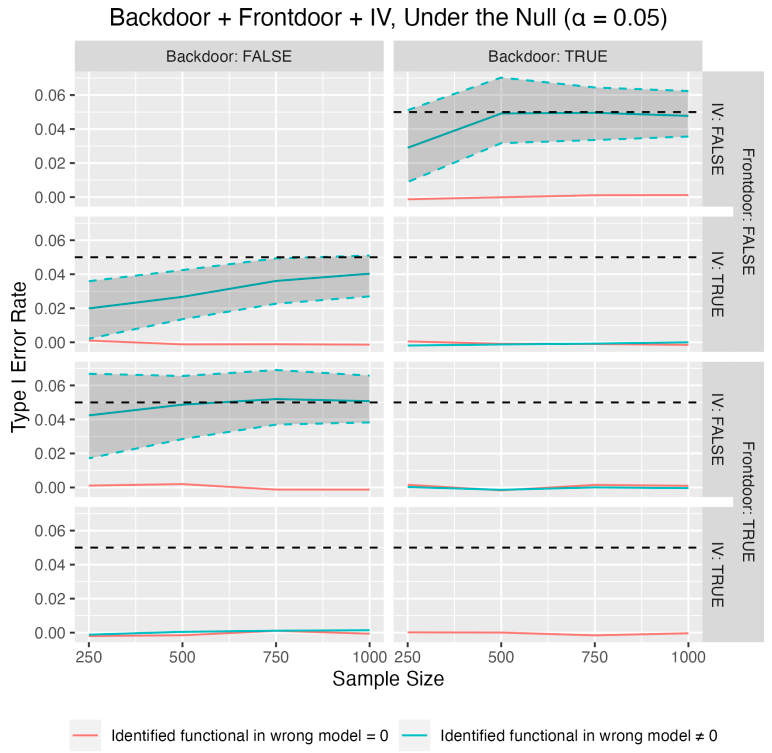
\includegraphics[scale=4]{calibration.pdf}
		% 		\caption{}
		% 	\end{subfigure}
		% 	\begin{subfigure}{\textwidth}
		% 		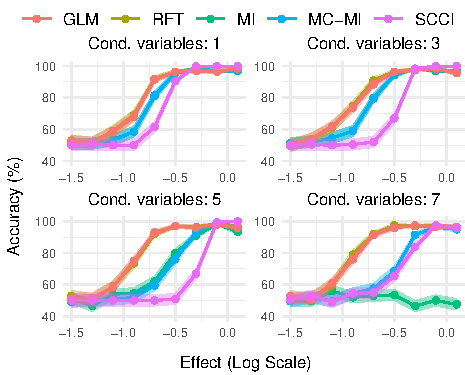
\includegraphics[scale=4]{accuracy.pdf}
		% 		\caption{}
		% 	\end{subfigure}
		% \end{figure}
		\begin{figure}
			\includegraphics[scale=3]{conclusion.pdf}
		\end{figure}

	\end{myblock}\vfill
	\begin{myblock}{Conclusion and Future Work}
		\begin{itemize}
			\item Shows the connection between path coefficients and effect sizes.
			\item Gives an effect size based on Canonical correlations for mixed data.
			\item Future work: How to interpret these coefficients.
			\item Future work: More analysis on the CI test based on this.
			\item Theoretical guarantees for the test needs to be derived.
		\end{itemize}
	\end{myblock}\vfill
	\begin{myblock}{References}
		\footnotesize
		\bibliography{./bib}
	\end{myblock}\vfill
		}\end{minipage}\end{beamercolorbox}
	\end{column}
\end{columns}
\end{frame}
\end{document}
